\documentclass[french]{amu_these}

\usepackage{bm}
\usepackage{physics}

\newcommand{\E}[1]{\mathbb{E} \left[{#1}\right]}
\newcommand{\Eq}[1]{Eq.~\ref{#1}}
\newcommand{\Eqs}[1]{Eqs.~\ref{#1}}
\newcommand{\Fig}[1]{Fig.~\ref{#1}}
\newcommand{\Figs}[1]{Figs.~\ref{#1}}
\newcommand{\avg}[1]{\left \langle #1 \right \rangle}

\begin{document}
						
	\chead{}
\pdfbookmark[0]{Page de titre}{titre}
\thispagestyle{empty}
\newgeometry{margin=2em}
% \newgeometry{left=3em,right=2em,top=2em,bottom=2em} %% marge pour la reliure en cas d'exemplaire imprimé

\vspace{1em}

\begin{center}
	\begin{minipage}[c]{.5\linewidth}
		\raggedright\includegraphics[height=7em]{logo_amu}
	\end{minipage}\hfill
	\begin{minipage}[c]{.5\linewidth}
		%\raggedleft\includegraphics[height=7em]{example-image-b} %% logo établissement en cotutelle, le cas échéant
	\end{minipage}\hfill
\end{center}

%\vspace{.4em}

\begin{center}
	\begin{minipage}[c]{.77\linewidth}
		\textcolor{yellowamu}{\noindent\rule{\textwidth}{4pt}}
	\end{minipage}\hfill
	\begin{minipage}[c]{.23\linewidth}
		\raggedleft\textsf{NNT : 2024AIXM0001}
		% renseigner votre numéro national de thèse (NNT)
	\end{minipage}\hfill
\end{center}

%\vspace{1em}

\doublespacing
\begin{flushleft}
    \textsf{\HUGE\textcolor{blueamu}{THÈSE DE DOCTORAT}}\\
	\textsf{\Large Soutenue à AMU ― Aix-Marseille Université}\\
	%\textsf{\Large dans le cadre d'une cotutelle avec }\\ %% établissement en cotutelle, le cas échéant
	\textsf{\Large le 10 janvier 2024 par}\\
\end{flushleft}
\vspace{2em}
\begin{center}
	\textsf{\textbf{\Huge Andonis Gerardos}}\\
    \vspace{1em}
	\textsf{\LARGE Model selection for noisy dynamical data:}\\ 
	\textsf{\Large A parsimonious and principled approach}\\
\end{center}
\singlespacing

\vspace{4em}

\begin{center}
	\begin{minipage}[t]{.45\linewidth}
    	    \vspace{.5em}
        	\textsf{\textbf{Discipline}}
        	
        	\textsf{Liste des disciplines en \hyperref[chap:doctorats]{annexe A}}
        	
    	    \vspace{1em}
        	\textsf{\textbf{Spécialité}}
        	
        	\textsf{Liste des spécialités en \hyperref[chap:doctorats]{annexe A}}
        	
    	    \vspace{2em}
        	\textsf{\textbf{École doctorale}}
        	
        	\textsf{ED 352 PHYSIQUE ET SCIENCES DE LA MATIERE : Biophysique}
        	
    	    \vspace{1em}
        	\textsf{\textbf{CINaM}}
        	
        	\textsf{CENTURI\\
        	ANR
        	}

    	    \vspace{3em}
        	\textsf{Consignes de présentation détaillées\\
			des pages liminaires en \hyperref[chap:consignes]{annexe B}}
	\end{minipage}\hfill
	\begin{minipage}[t]{.03\linewidth}
	    \rule[-280pt]{1pt}{280pt}
	\end{minipage}\hfill
	\begin{minipage}[t]{.52\linewidth}
	    \vspace{.5em}
    	\textsf{\textbf{Composition du jury}}

	    \vspace{1em}
    	\textsf{
        \begin{tabular}{p{12em} p{10em}}
        	Prénom NOM & Rapporteur·e \\
        	Titre et affiliation \\
        	\\
        	Prénom NOM & Rapporteur·e \\
        	Titre et affiliation \\
            \\
            Prénom NOM & Examinateur·rice \\
        	Titre et affiliation \\
            \\
        	Prénom NOM & Président·e du jury \\
        	Titre et affiliation \\
            \\
        	Prénom NOM & Directeur·rice de thèse \\
        	Titre et affiliation \\
           \\
        	Prénom NOM & Membre invité·e \\
        	Titre et affiliation \\
        \end{tabular}
        }
	\end{minipage}\hfill
\end{center}       

\vspace{2em}

\begin{center} %% logos partenaires
	\begin{minipage}[c]{.25\linewidth}
		\centering
\includegraphics[height=10em]{logo/logo-CENTURI.png} 
	\end{minipage}\hfill
	\begin{minipage}[c]{.25\linewidth}
		\centering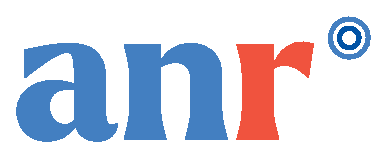
\includegraphics[height=5em]{logo/ANR-logo-2021-sigle.eps}
	\end{minipage}\hfill
	\begin{minipage}[c]{.25\linewidth}
		\centering
\includegraphics[height=5em]{logo/logo-cinam.png} 
	\end{minipage}\hfill
	\begin{minipage}[c]{.25\linewidth}
	\end{minipage}\hfill
\end{center}

\restoregeometry
				%% page de titre
										
	\newpage
\addchap{Affidavit}
\label{chap:affidavit}
\thispagestyle{empty}

\iftrue % Déclaration sur l'honneur pour une thèse en français (inverser les \if pour une thèse en anglais)
    Je soussigné, Andonis Gerardos, %% Prénom et Nom de l'auteur %%
    déclare par la présente que le travail présenté dans ce manuscrit est mon propre travail, réalisé sous la direction scientifique de Pierre Ronceray, % Prénom et Nom du directeur de thèse et s’il y a lieu du co-directeur de thèse
    dans le respect des principes d’honnêteté, d'intégrité et de responsabilité inhérents à la mission de recherche. Les travaux de recherche et la rédaction de ce manuscrit ont été réalisés dans le respect à la fois de la charte nationale de déontologie des métiers de la recherche et de la charte AMU relative à la lutte contre le plagiat.
    
    Ce travail n'a pas été précédemment soumis en France ou à l'étranger dans une version identique ou similaire à un organisme examinateur.\\
    
    Fait à Marseille le 01/04/2025
    
    \begin{flushright}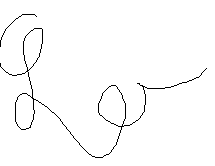
\includegraphics[width=120px,height=40px]{logo/signature.png}\end{flushright}% signature

    ~\vfill
    \begin{center}
        \begin{minipage}[c]{0.25\linewidth}
            \includegraphics[height=35px]{by-nc-nd-eu}
        \end{minipage}\hfill
    \end{center}

    Cette \oe{}uvre est mise à disposition selon les termes de la \href{https://creativecommons.org/licenses/by-nc-nd/4.0/deed.fr}{Licence Creative Commons Attribution - Pas d’Utilisation Commerciale - Pas de Modification 4.0 International}. % consultez les conditions de la licence cc by-nc-nd, vous pouvez appliquer une licence moins restrictive, cc by-nc-sa par exemple
\fi

\iffalse % Affidavit of Honour for english thesis (invert the \if for an English thesis)
    I, undersigned, Andonis Gerardos, %% First Name and Surname of the PhD student
    hereby declare that the work presented in this manuscript is my own work, carried out under the scientific supervision of Pierre Ronceray, %% First Name and Surname of the thesis director and if applicable of the co-thesis director
    in accordance with the principles of honesty, integrity and responsibility inherent to the research mission. The research work and the writing of this manuscript have been carried out in compliance with both the french national charter for Research Integrity and AMU charter on the fight against plagiarism.
    
    This work has not been submitted previously either in this country or in another country in the same or in a similar version to any other examination body.\\
    
    Marseille 01/04/2025
    
    \begin{flushright}\includegraphics[width=120px,height=40px]{example-image-a}\end{flushright}% signature

    ~\vfill
    \begin{center}
        \begin{minipage}[c]{0.25\linewidth}
            \includegraphics[height=35px]{by-nc-nd-eu}
        \end{minipage}\hfill
    \end{center}

    This work is licensed under \href{https://creativecommons.org/licenses/by-nc-nd/4.0/deed.en}{Creative Commons Attribution-NonCommercial-NoDerivatives 4.0 International Public License}
\fi

				%% affidavit et licence

	\input{tex_before/publications}			%% liste de publications et participation aux conférences

	\input{tex_before/resume}					%% résumé

	\input{tex_before/abstract}				%% abstract

	\input{tex_before/remercie}				%% remerciements

    \microtypesetup{protrusion=false}	%% désactive la protrusion (TOC LOFT GLS)
	\tableofcontents					%% TOC
	\listoffigures						%% LOF
	\listoftables						%% LOT
	\printglossary[						%% acronymes
		type=\acronymtype,
		title={Liste des acronymes},
		toctitle={Liste des acronymes}
		]
	\printglossary[						%% glossaire
		title={Glossaire},
		toctitle={Glossaire}
		]
	\printglossary[						%% nomenclature
		type=notation,
		title={Nomenclature},
		toctitle={Nomenclature}
		]
    \microtypesetup{protrusion=true}	%% rétabli la protrusion

	\ohead{\leftmark\Ifstr{\rightmark}{\leftmark}{}{ -- \rightmark}}	%% place le chapître et la partie en en-tête

	\addchap{Introduction}

\section{General Context}

\section{Motivations and Problems}
\subsection{Challenges in Inference}
Discuss the challenges encountered in inference, such as measurement noise and large sampling intervals.

\subsection{Need for Robust Model Selection}
Explain the necessity for robust methods to select parsimonious models.

\section{Objectives and Contributions of the Thesis}
\begin{itemize}
    \item Development of two robust techniques for the inference of SDE/SPDE.
    \item Proposal of a model comparison method based on Wilks’ theorem and large deviation calculations.
\end{itemize}

\section{Outline of the Manuscript}
Provide a brief overview of the following chapters.


	\chapter{Theoretical Framework and State of the Art}
\chaptertoc{}

\section{Introduction to SDE and SPDE}
Recap the theoretical foundations, definitions, and key properties of SDE and SPDE.

\section{Existing Inference Techniques}
Review common methods, their advantages, and limitations—especially regarding measurement noise and sampling issues.

\section{Model Selection Criteria}
Present existing approaches, the role of Wilks’ theorem, and the principles of large deviations in statistics.

\section{Positioning of Your Work}
Explain how your contributions fit into the broader context of the field.


				\begin{figure}
					\centering
					\subfloat[Figure A]{\includegraphics[width=.5\textwidth, max height=2in]{example-image-a}}
					\subfloat[Figure B]{\includegraphics[width=.5\textwidth, max height=2in]{example-image-b}}
					\caption{Deux figures}
					\label{fig:deux_figures}
				\end{figure}



	\chapter{Techniques to Improve SDE/SPDE Inference}
\chaptertoc{}

\section{Presentation of Practical Challenges}

When acquiring any type of data, an experimentalist has to face two challenges among several others. The first is the time between two measurements, called the sampling time, which we would like to be as small as possible. However, many practical issues constrain the sampling time. As an example, fluorescent proteins used to image the biological object of interest lose their fluorescent properties when acquiring several different images. Thus, for fluorescent proteins, increasing the sampling time is particularly interesting for increasing the observation time. The second issue is the measurement error, defined as the difference between a measured value of a quantity and its unknown true value. Any measurement has its inherent measurement error. Thus, it is very important that any inference method is robust to measurement noise.

\begin{figure}
    \centering
    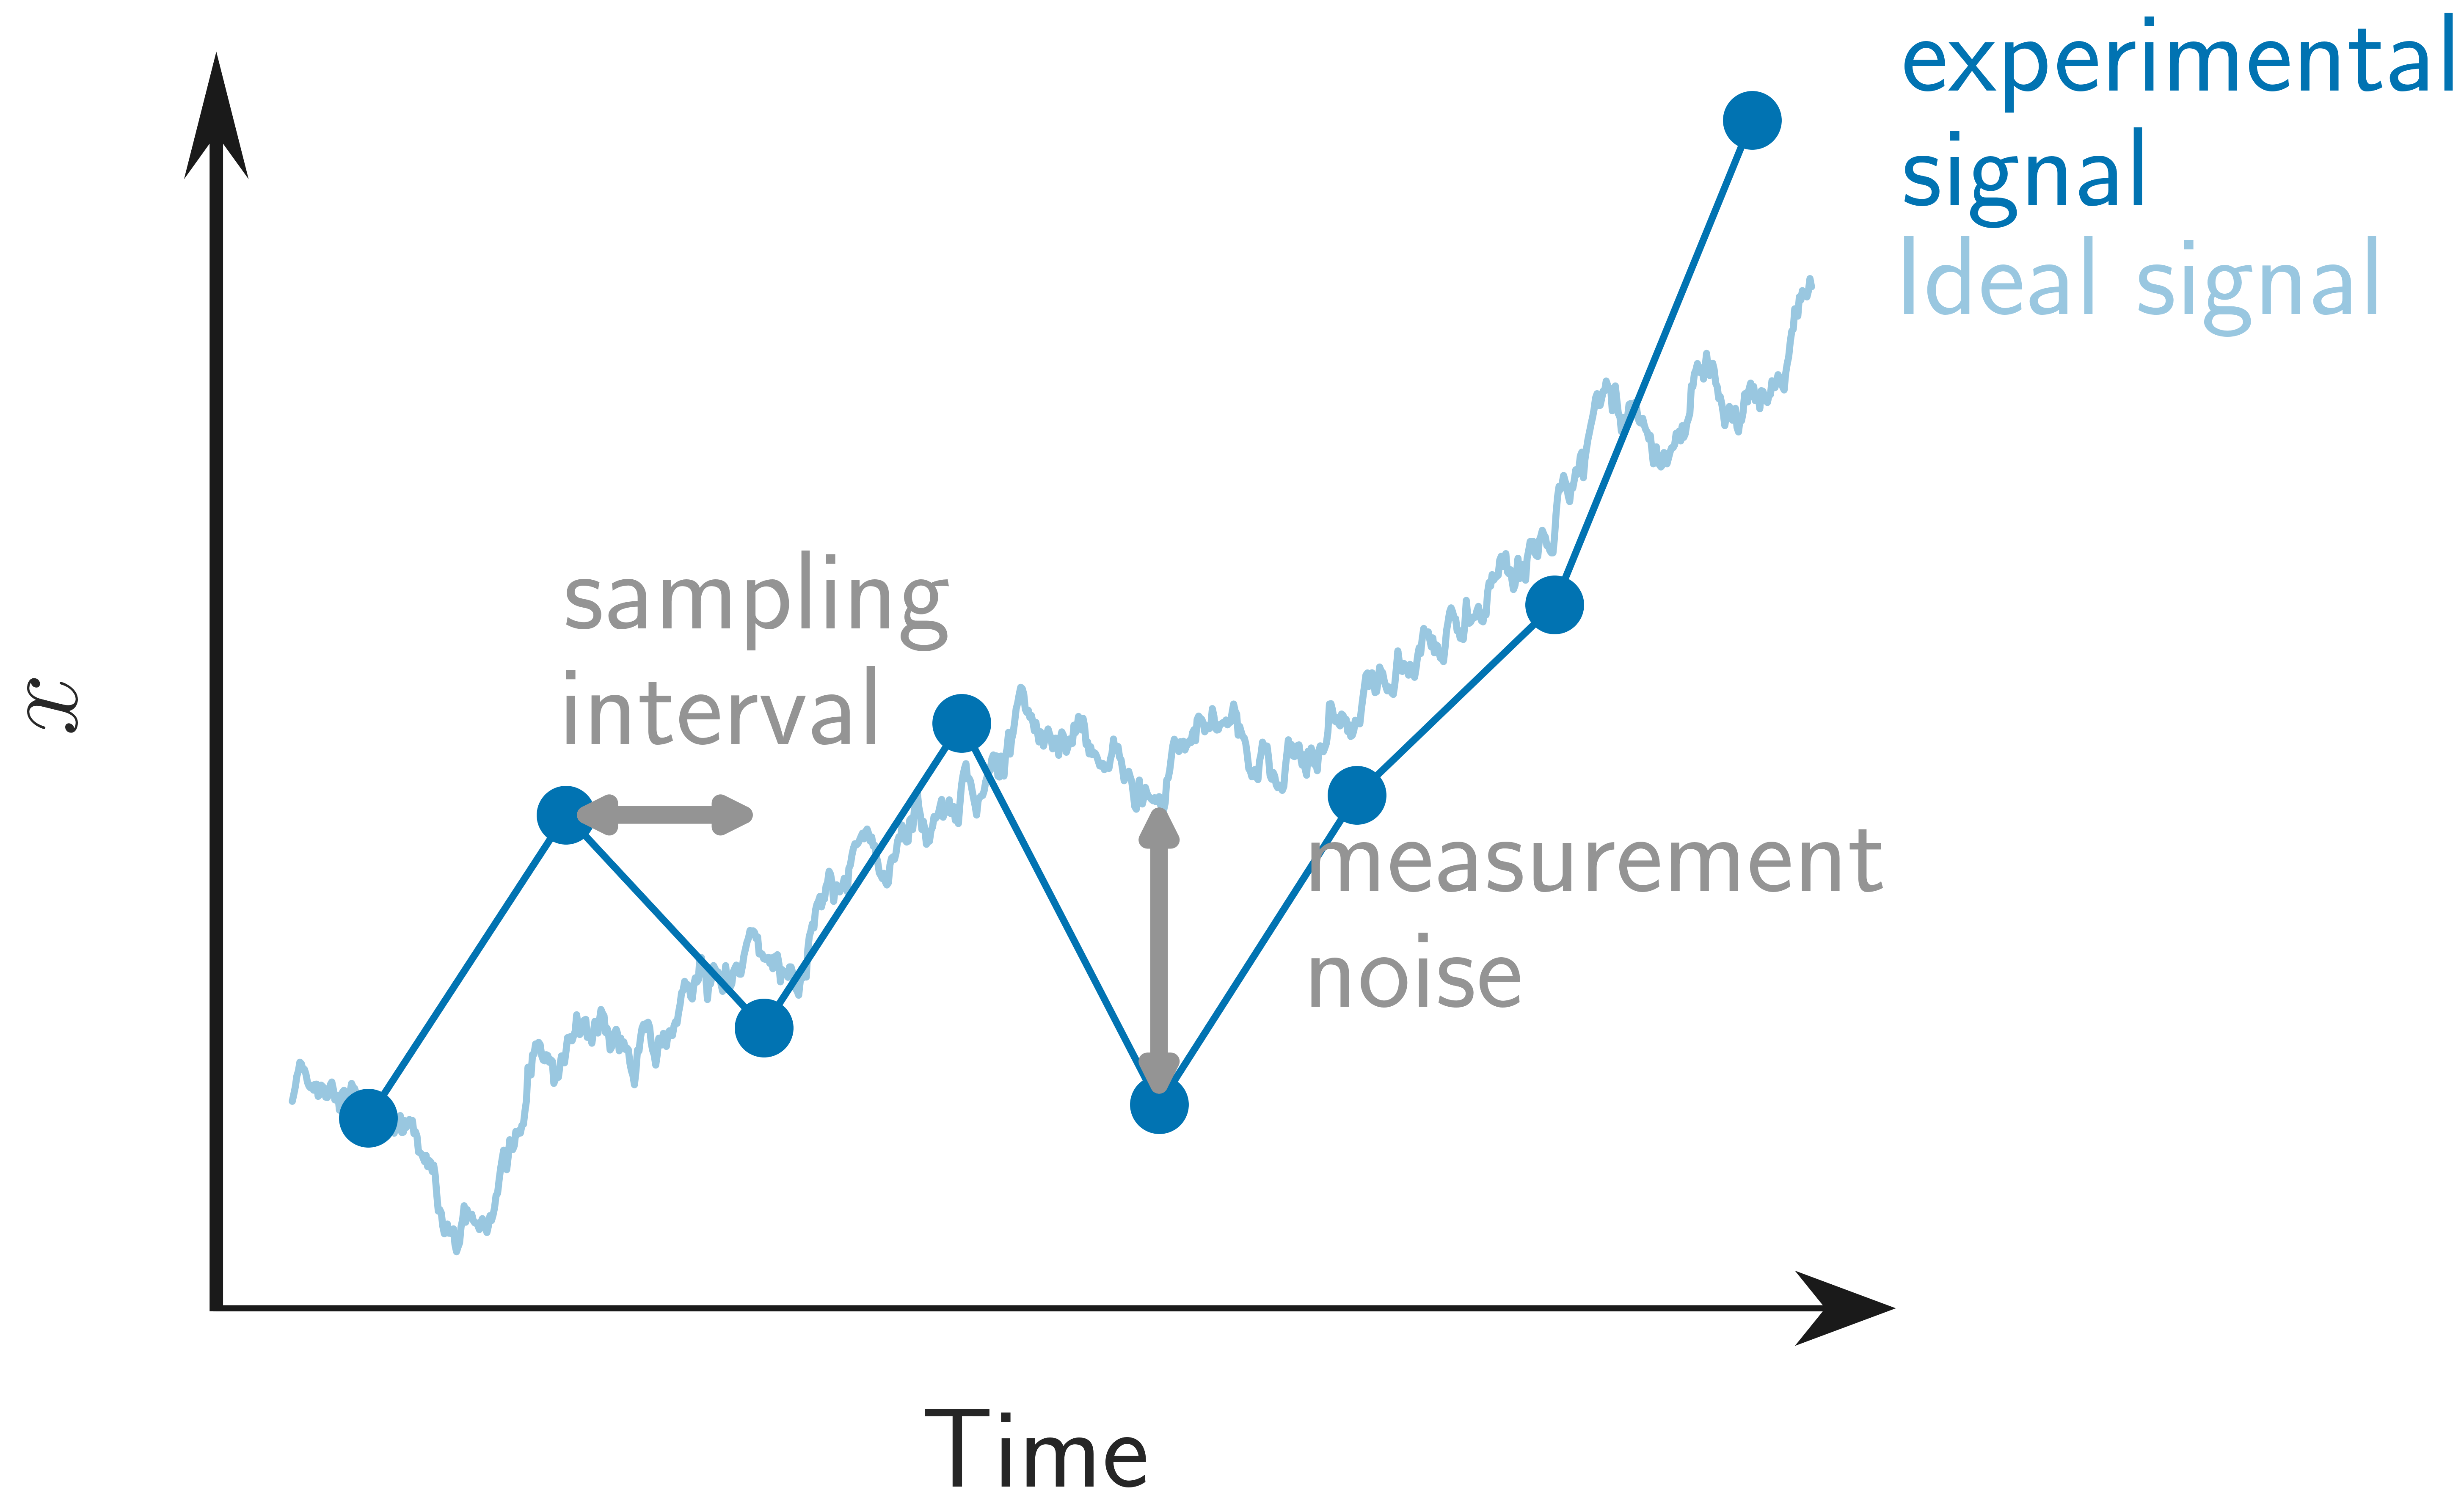
\includegraphics[width=0.5\linewidth]{fig/illustration_signal_2.png}
    \caption{Schema of the measured expiremental signal versus the real signal, which is impacted by sampling interval and measurement noise.}
    \label{fig:enter-label}
\end{figure}

\section{Robustness with Large Sampling Intervals}
In the previous chapter, we derived an estimator for the drift that uses the assumption $\frac{\Delta \bm{x_t}}{\Delta t} \approx \bm{f}(\bm{x_t})$ which relies on the sampling interval $\Delta t \to 0$. What is going to happen to the drift estimator if $\Delta t \to 0$ ? To answer this question, we need to take a look at 
\begin{equation}
    \frac{\Delta\bm{x_t}}{\Delta t} = \frac{1}{\Delta t}\int_t^{t+\Delta t} \left(\bm{f}(\bm{x_{t'}}) + \bm{\xi_{t'}} \right)\dd{t'}
    \label{eq:delta_x}
\end{equation}. To understand its behavior when $\Delta t$ increases, we Taylor expand $\bm{f}(\bm{x_{t'}})$ around $\bm{x_t}$ :
\begin{align}
    \bm{f}(\bm{x_{t'}}) &= \bm{f}(\bm{x_t}) + (\bm{x_t'} - \bm{x_{t}}).\nabla \bm{f}(\bm{x_t}) + \bm{D(x_t)}.\nabla^2\bm{f}(\bm{x_t}) (t'-t) + O(\Delta t^2) + O_\text{fluc}(\Delta t^{3/2})\\
    &= \bm{f}(\bm{x_t}) + \underbrace{\left(\bm{f}(\bm{x_t}).\nabla \bm{f}(\bm{x_t}) + \bm{D(x_t)}.\nabla^2\bm{f}(\bm{x_t})\right)}_{\bm{A}} (t'-t)  +O(\Delta t^2) + O_\text{fluc}(\Delta t^{1/2})
    \label{eq:Taylor_b}
\end{align}
where $\bm{D(x_t)}.\nabla^2\bm{f}(\bm{x_t})  = \sum_{\beta, \gamma} D_{\beta\gamma}(\bm{x_t})\pdv{\bm{f}}{x_{\beta}}{x_{\gamma}}$ and $O_\text{fluc}(\Delta t^{3/2})$ contains fluctuating terms such as $\int_t^{t+\Delta t}\bm{f(x_{t'})} \dd{t'} \int_t^{t+\Delta t}\bm{\xi_{t'}} \dd{t'}$ and higher orders. Thus, a more appropriate formulation for large sampling interval is $\frac{\Delta\bm{x_t}}{\Delta t} = \bm{f}(\bm{x_t}) + \bm{A} \frac{\Delta t}{2} + O(\Delta t^2) + O_\text{fluc}(\Delta t^{-1/2})$. But, by choosing $t'= t + \Delta t$ in \Eq{eq:Taylor_b}, we realize that $\bm{A} \approx \frac{\bm{f}(\bm{x_{t+ \Delta t})} - \bm{f}(\bm{x_t)}}{\Delta t}$ which leads to :
\begin{equation}
    \frac{\Delta\bm{x_t}}{\Delta t} = \frac{\bm{f}(\bm{x_{t+\Delta t})} + \bm{f}(\bm{x_t)}}{2}  + O(\Delta t^2) + O_\text{fluc}(\Delta t^{-1/2})
    \label{eq:delta_x_trapeze}
\end{equation}
So finally, we demonstrated that the trapeze formulation works for SDE integral. Wouaahhh, amazing. The interesting thing is to leverage this knowledge to improve the robustness of our drift estimator. To do so, we suppose that there exists a function base $\mathcal{B} = \{\bm{b_i}\}_{i=1,n}$ where $\bm{f}$ can be decomposed on such that : $\bm{f}(\bm{x}) = \sum_i \alpha_i\bm{b}_i(\bm{x})$. By multiplying \Eq{eq:delta_x_trapeze} by $\bm{b_i} \frac{\bm{\bar{D}}^{-1}}{4}$ and averaging over time, we get a simple equation 
\begin{equation}
    \avg{\frac{\Delta\bm{x_t}}{\Delta t}\cdot \frac{\bm{\bar{D}}^{-1}}{4}\bm{b_i}(\bm{x_t)}} = \sum_j \underbrace{\avg{\frac{\bm{b_j(x_t)} + \bm{b_j(x_{t+\Delta t})}}{2} \cdot \bm{\bar{D}}^{-1}\bm{b_i(x_t)}}}_{\left(G_{\mathcal{B}}^{Tr}\right)_{ij}} \alpha_j 
    \label{eq:chap_1_alpha_trapeze}
\end{equation}
which we can invert to obtain the learned parameters $\hat{\alpha_i}^{Tr}$
\begin{equation}
    \hat{\alpha_i}^{Tr} = \sum_j \left(G_{\mathcal{B}}^{Tr}\right)^{-1}_{ij} \avg{\frac{\Delta\bm{x_t}}{\Delta t}\cdot \bm{\bar{D}}^{-1}\bm{b_j}(\bm{x_t)}}
\end{equation}
Note that this estimator doesn't derive from the maximization of a likelihood function but when $\Delta t \to 0$, $\hat{\alpha_i}^{Tr}\to \hat{\alpha_i}$ which is a likelihood estimator. From the previous derivation, we expect that the reconstructed drift with $\hat{\alpha}_i$ has an error in $O(\Delta t)$ but for the reconstructed drift with the trapeze formulation $\hat{\alpha_i}^{Tr}$ we expect to have an error in $O(\Delta t^2)$. Indeed, we observe this behavior in \Fig{fig:Lorenz_benchmark}. This work leads to co-publication in~\cite{amiriInferringGeometricalDynamics2024}. Note that, I discovered recently that another PhD student was working on the same question and obtained the same trapeze estimator but with a different demonstration in~\cite{wannerHigherOrderDrift2024}.

\begin{figure}
    \centering
    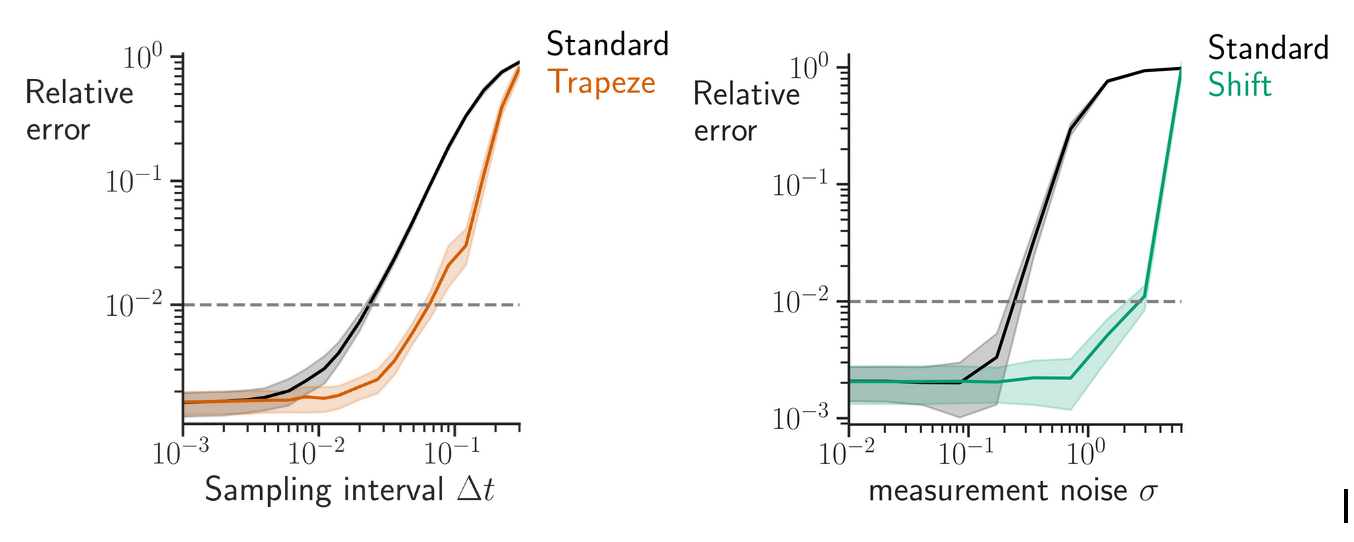
\includegraphics[width=0.5\linewidth]{fig/Lorenz_sampling_measurement noise_benchmark.png}
    \caption{NEED TO be done}
    \label{fig:Lorenz_benchmark}
\end{figure}












\section{Robustness Against Measurement Noise}

Measurement noise can be decomposed into two categories: the systematic error which always occurs with the same value (for instance, a wrongly calibrated balance), and the random error that varies from one observation to another. Here, we are only considering the random error by modeling the measurement noise as a Gaussian random variable which is added to the true trajectory $\bm{x_t} \rightarrow \bm{x_t} + \bm{\eta_t}$ with $\bm{\eta_t} \sim \mathcal{N}(0, \bm{\sigma})$. This simple measurement noise is going to affect our inferred drift. How ? Let us look at our estimator for the instantaneous drift $\frac{\Delta \bm{x_t}}{\Delta{t}} \rightarrow \frac{\Delta \bm{x_t}}{\Delta{t}} + \frac{\Delta \bm{\eta_t}}{\Delta{t}}$. From that, we see the dramatic coupling between the measurement noise and sampling interval: the standard deviation of the measurement noise is amplified by a prefactor $\frac{1}{\Delta t}$ which can be considerably big. Thus, when we infer the drift using the average : 
\begin{equation}
    \avg{\left(\frac{\Delta \bm{x_t}}{\Delta{t}} + \frac{\Delta \bm{\eta_t}}{\Delta{t}}\right)\cdot \frac{\bm{\bar{D}}^{-1}}{4}\bm{b_j}\left(\bm{x_t + \eta_t}\right)} = \avg{\frac{\Delta \bm{x_t}}{\Delta{t}} \cdot \frac{\bm{\bar{D}}^{-1}}{4}\bm{b_j}\left(\bm{x_t + \eta_t}\right)} + \avg{\frac{\Delta \bm{\eta_t}}{\Delta{t}}\cdot \frac{\bm{\bar{D}}^{-1}}{4}\bm{b_j}\left(\bm{x_t + \eta_t}\right)}
\end{equation}
the term $\avg{\frac{\Delta \bm{\eta_t}}{\Delta{t}}\cdot \frac{\bm{\bar{D}}^{-1}}{4}\bm{b_j}\left(\bm{x_t + \eta_t}\right)}$ is of order $\frac{\sigma^2}{\Delta t}$ and it is going to strongly bias our inference. We need a way to ensure this term to average to zero. How can we do that ? One way is to average over $\bm{b_j}(\bm{x_{t-\Delta t}})$ instead of $\bm{b_j}(\bm{x_t})$. Thus, we obtain : 

\begin{multline*}
    \avg{\left(\frac{\Delta \bm{x_t}}{\Delta{t}} + \frac{\Delta \bm{\eta_t}}{\Delta{t}}\right)\cdot \frac{\bm{\bar{D}}^{-1}}{4}\bm{b_j}\left(\bm{x_{t-\Delta t} + \eta_{t-\Delta t}}\right)} = \avg{\frac{\Delta \bm{x_{t}}}{\Delta{t}} \cdot \frac{\bm{\bar{D}}^{-1}}{4}\bm{b_j}\left(\bm{x_{t-\Delta t} + \eta_{t-\Delta t}}\right)} \\
    + \avg{\frac{\Delta \bm{\eta_t}}{\Delta{t}}\cdot \frac{\bm{\bar{D}}^{-1}}{4}\bm{b_j}\left(\bm{x_{t-\Delta t} + \eta_{t-\Delta t}}\right)}
\end{multline*}


\section{Comparative Discussion of Both Techniques}
Evaluate the advantages, limitations, and optimal conditions for each method.




	\chapter{Comparison and Selection of Parsimonious Models}
\chaptertoc{}


\section{The Problem of Model Selection}
Discuss the necessity of an approach that selects the simplest model without compromising performance.

\section{Theoretical Foundations of the Proposed Method}
\subsection{Wilks' Theorem in this Context}
Present the application of Wilks' theorem to the model selection problem.

\subsection{Role of Large Deviation Calculations}
Explain how large deviation calculations are used for performance evaluation.

\section{Development of the Method}
\subsection{Theoretical Derivations}
Detail the theoretical derivations underpinning the method.

\subsection{Implementation Details and Algorithms}
Provide the algorithmic implementation and practical details.

\section{Numerical Studies and Comparison with Existing Methods}
\subsection{Presentation of Simulation Results}
Show the results obtained from simulations.

\subsection{Discussion on Robustness and Efficiency}
Discuss the robustness and efficiency of the proposed method compared to existing techniques.

\section{Interpretations and Implications}
Consider the impact on model selection in similar contexts and potential generalizations.


	\addchap{Conclusion}
\section{Interpretations and Implications}
Consider the impact on model selection in similar contexts and potential generalizations.

	\appendix

	\newpage
	\printbibliography[heading=bibintoc]%% bibliographie
	
	\newpage
	\printindex							%% index
	
	\newpage
	\printendnotes						%% notes

	%\setcounter{chapter}{0}
%\renewcommand{\thesection}{\Alph{section}}

\addpart{ANNEXES}

\input{tex_behind/annexe1}
% \input{tex_behind/annexe2}
% \input{tex_behind/annexe3}			%% annexes

\end{document}
